\documentclass[14pt,a4paper]{scrartcl}
\usepackage[utf8]{inputenc}
\usepackage[english,russian,ukrainian]{babel}
\usepackage{indentfirst}
\usepackage{misccorr}
\usepackage{graphicx}
\usepackage{xcolor}
\usepackage{cmap}
\usepackage{amsmath,amsfonts,amssymb,amsthm,mathtools}
\usepackage{icomma}
\usepackage{multirow}
\usepackage{geometry} \geometry{verbose,a4paper,tmargin=1cm,bmargin=2.5 cm,lmargin=2cm,rmargin=1cm}
\usepackage{euscript}
\usepackage{mathrsfs}
\usepackage{mathtext}
\usepackage{graphicx}
\usepackage{booktabs}
\usepackage{color}
\usepackage{rotating}
\usepackage{pdflscape}
\usepackage{floatrow}
\usepackage{subcaption}
\usepackage{calc}
\linespread{1.3}
\setlength{\parindent}{5ex}


\begin{document}

\pagecolor{white}
\begin{titlepage}
  \begin{center}
    \large
    Національний технічний університет України \\ "Київський політехнічний інститут імені Ігоря Сікорського"
     
       
    Факультет Електроніки
     
    Кафедра мікроелектроніки
    \vfill
      
    \textsc{ЗВІТ}\\
     
    {\Large Про виконання лабораторної роботи №3\\
      з дисципліни: «Схемотехніка-1. Аналогова схемотехніка»\\[1cm]
      
    {\bf ОПЕРАЦІЙНІ ЛАНКИ НУЛЬОВОГО ПОРЯДКУ}\\
    
    }
  \bigskip
\end{center}
\vfill
 
\newlength{\ML}
\settowidth{\ML}{«\underline{\hspace{0.4cm}}» \underline{\hspace{2cm}}}
\hfill
\begin{minipage}{1\textwidth}
Виконав:\\
Студент 3-го курсу \hspace{4cm} $\underset{\text{(підпис)}}{\underline{\hspace{0.2\textwidth}}}$  \hspace{1cm}Кузьмінський О.Р.\\
\vspace{1cm}

Перевірила: \hspace{6.1cm} $\underset{\text{(підпис)}}{\underline{\hspace{0.2\textwidth}}}$  \hspace{1 cm}Бевза О.М.\\

\end{minipage}

\vfill

\begin{center}
2021
\end{center}
\end{titlepage}

\begin{center}
{\Large 1.Мета завдання}
\end{center}

Вивчення принципів роботи, дослідження амплітудних
характеристик та параметрів різних функціональних ланок на основі
інтегральних операційних підсилювачів (інвертуючого та неінвертуючого
підсилювачів, сумуючого та віднімаючого підсилювачів).

\begin{center}
{\Large 2.Порядок виконання завдання}
\end{center}

\begin{enumerate}
\item Включити лабораторну установку для дослідження
операційних ланок нульового порядку. Підключити лабораторну установку
відповідно до блок-схеми(рис.1).
\item Для схем масштабного підсилювача з інвертування та без
інвертування:
\begin{enumerate}
\item Виміряти вхідний $R_{\text{вх}}$ та вихідний опір $R_{\text{вих}}$, коефіцієнт
передачі напруги $K_U$ при підключенні опорів $R_1$ та $R_4$ і
$U_{\text{вх}}$=$U_1$ =0,1 В на частоті $f_{\text{г}}=1$ кГц.

\item Обчислити коефіцієнти передачі напруги $K_U=\dfrac{U_2}{U_1}$, струму $K_I=\dfrac{R_{\text{вх}}}{R_4}K_U$, та потужності $K_P=K_U\times{K_I}$
\item Визначити максимальну частоту масштабних підсилювачів при припустимому зменшенні коефіцієнта передачі до рівня \\
$M_{\text{д}}=\dfrac{K_U(f_{\text{в}})}{K_U(f_0=1 \text{кГц}=0,707)}$
\item Змалювати з екрана осцилографа та порівняти амплітуди
і фази напруг $U_1$ та $U_2$.
\item Результат вимірювань та осцилограми внести в табл. 3.2.
\item Виміряти та побудувати графік амплітудної характеристики $U_2 =U_2 (U_1)$
неінвертуючого підсилювача (П2) на частоті $f_{\text{г}}=1$ кГц. Відзначити знаками «+» і «–» відповідно найбільше значення вхідної напруги $U_1$($U_{1max}^+$ та $U_{1max}^-$), при яких з'являються помітні нелінійні спотворення вихідної напруги $U_2$
позитивної та негативної полярності. Обчислити динамічний діапазон вхідного напруги позитивної $\text{Д}^+$ та негативної $\text{Д}^-$ полярностей:
$\text{Д}^+=\dfrac{U_{1max}^+}{U_{1min}}$, де $U_{1min}$-мінімальна амплітуда вхідної напруги, помітна на рівні шумів при заданому відношенні 
$\dfrac{\text{сигнал}}{\text{шум}}$(взяти $\dfrac{\text{сигнал}}{\text{шум}}=3$).
\end{enumerate}
\item Для диференціального масштабного підсилювача, інвертуючого та неінвертуючого сумуючих підсилювачів змалювати осцилограми вхідних напруг ($U_{11}=U_{\text{г}}, U_{12}$) та вихідної напруги ($U_2$) на частоті $f_{\text{г}}=1$ кГц, $U_{11m}=1$ В, де : $U_{11}(t)=U_{1m}\sin(\omega t+\phi)$ при $0\le t\le T$;\\

 $U_{11}$ знімається з виходу КТ3,\\

$U_{12}(t)=
\begin{cases}
1& \text{при } t_1\le t\le (t_1+t_u)\\
0& \text{при} (t_1+t_u)\le t\le (t_1+t_u+t_n)
\end{cases}
$-знімається з виходу КТ7,\\

$U_2$ знімається з виходу КТ3.\\

Для зазначених трьох підсилювачів (ДМП, ІСП, НСП) записати
аналітичний вираз для вихідної напруги $U_2(t)$ у символьному вигляді та
чисельно і порівняти результати вимірювань з розрахунками, зробити
висновки по кожному пункту досліджень.\\
Тут $U_{1m}$--- амплітуда вхідного сигналу $U_{11}$, $U_{2m}$---максимальне значення вхідного сигналу $U_{12}$, T--- період вхідного сигналу $U_{11}$, $t_u$--- тривалість імпульсу вхідного сигналу $U_{12}$, $t_n$--- тривалість паузи вхідного сигналу $U_{12}$.
\item Визначити споживану потужність установки при проведенні
лабораторних досліджень, знаючи час проведення досліджень та
споживану потужність блоків установки.
\end{enumerate}
\medskip\hrule\medskip
\newpage 
\begin{center}
{\Large 3.Схеми вимірювання}
\end{center}

\begin{figure}[h]
\center{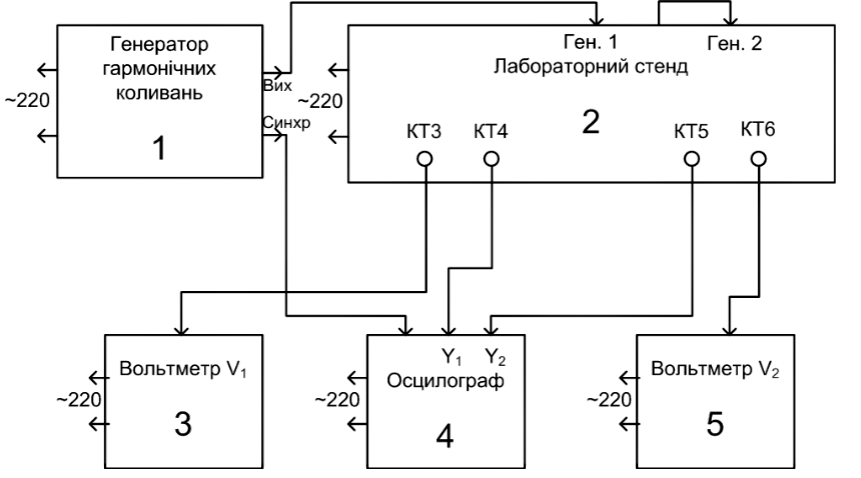
\includegraphics[width=0.5\textwidth]{op2}}
\caption{Блок-схема лабораторного макета «Операційні ланки нульовогопорядку».}
\end{figure}

\begin{figure}[h]
\center{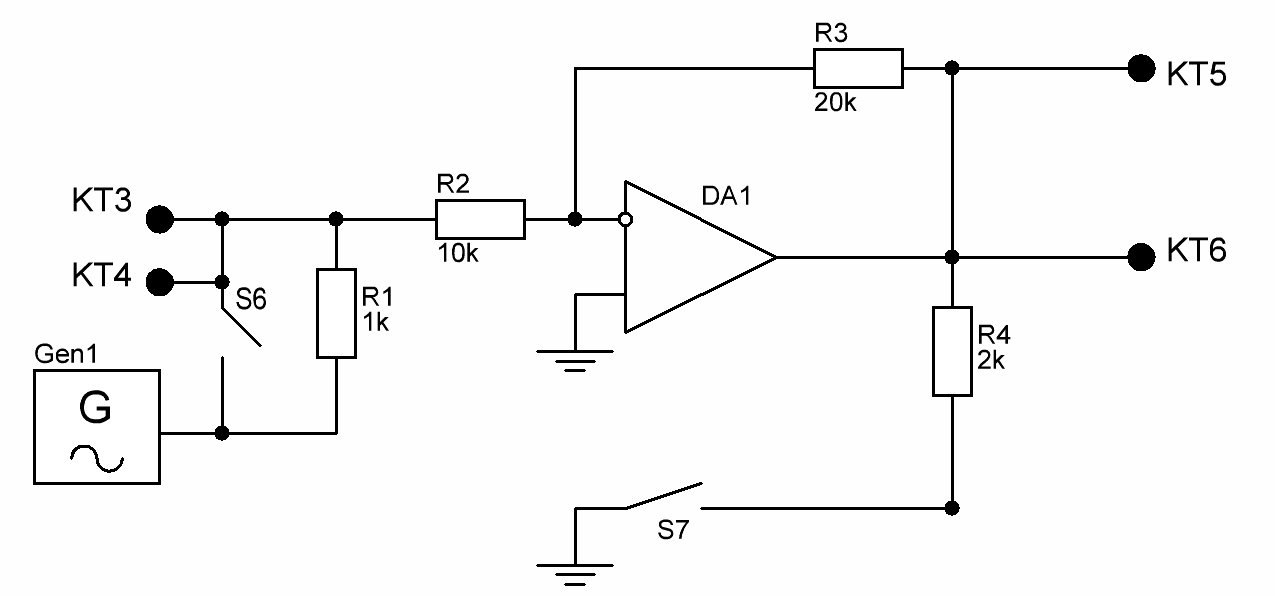
\includegraphics[width=0.5\textwidth]{op}}
\caption{ІМП}
\end{figure}

\begin{figure}[h]
\center{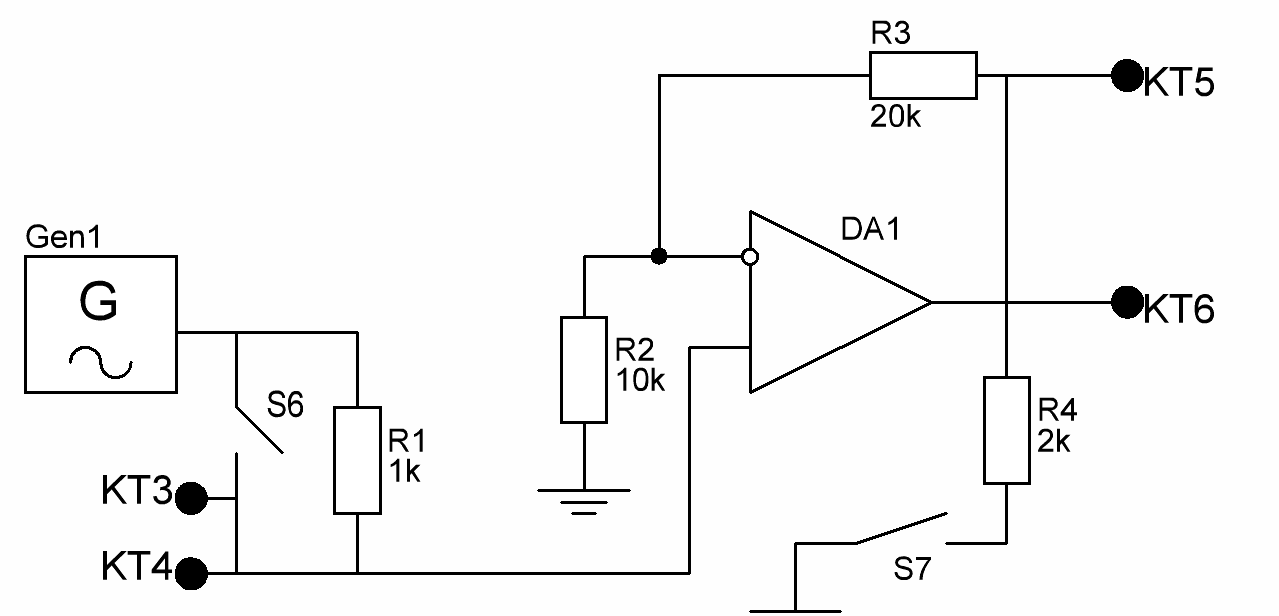
\includegraphics[width=0.5\textwidth]{op1}}
\caption{НМП}
\end{figure}
\newpage

\begin{center}
{\Large 4.Результати вимірювань}
\end{center}

\begin{center}
Табл.1. До вимірювань функцій масштабних підсилювачів (ІМП, НМП).\\[0.5cm]
\begin{tabular}{|l|l|l|l|}
\hline
\multicolumn{1}{|c|}{\multirow{2}{*}{№}} & \multirow{2}{*}{\begin{tabular}[c]{@{}l@{}}Показники роботи\\ підсилювача\end{tabular}}                    & \multicolumn{2}{c|}{\begin{tabular}[c]{@{}c@{}}Підсилювач в\\ схемі\end{tabular}}                                                                 \\ \cline{3-4} 
\multicolumn{1}{|c|}{}                   &                                                                                                            & \multicolumn{1}{c|}{\begin{tabular}[c]{@{}c@{}}ІМП\\ (П1)\end{tabular}} & \multicolumn{1}{c|}{\begin{tabular}[c]{@{}c@{}}НМП\\ (П2)\end{tabular}} \\ \hline
1                                        & \begin{tabular}[c]{@{}l@{}}При $R_1=0$\\ (П6-замкнутий) $U_{\text{г}}$,мВ\end{tabular}                     & 100                                                                     & 100                                                                     \\ \hline
2                                        & \begin{tabular}[c]{@{}l@{}}При $R_1=1$ кОм\\ (П6-розімкнений)\\ $U_1$, мВ\end{tabular}                     & 91,3                                                                    & 99,4                                                                    \\ \hline
3                                        & $R_{\text{вх}}=R_1\dfrac{U_1}{U_{\text{г}}-U_1}$                                                           & 10,49                                                                 & 165,7                                                                \\ \hline
4                                        & \begin{tabular}[c]{@{}l@{}}При $R_4=\infty$,\\ $U_{2xx}$, мВ\end{tabular}                                  & 199                                                                     & 300                                                                     \\ \hline
5                                        & \begin{tabular}[c]{@{}l@{}}При $R_4=2$ кОм,\\ $U_2$, мВ\end{tabular}                                       & 199                                                                     & 300                                                                     \\ \hline
6                                        & $R_{\text{вих}}=R_4\dfrac{U_{2xx-U_2}}{U_2}$, Ом                                                           & 0                                                                       & 0                                                                       \\ \hline
7                                        & $K_U=\dfrac{U_2}{U_1}$                                                                                     & 2,18                                                                  & 3,018                                                                  \\ \hline
8                                        & $K_I=K_U\dfrac{R_{\text{вх}}}{R_4}$                                                                        & 11,434                                                                 & 250,041                                                                \\ \hline
9                                        & $K_P=K_U\cdot{K_I}$                                                                                        & 24,926                                                                 & 754,624                                                                \\ \hline
10                                       & Епюри напруги $U_1$(---) та $U_2$(....)                                                                    & протифазні                                                             & синфазні                                                               \\ \hline
11                                       & \begin{tabular}[c]{@{}l@{}}$f_{\text{в}}=f_{max}$, кГц \\ при $U_{2\text{в}}=0,707\cdot{U_2}$\end{tabular} & 500-600                                                                 & 500-600                                                                 \\ \hline
\end{tabular}
\end{center}

\begin{center}
Табл.2. До вимірювань амплітудної характеристики неінвертуючого масштабного підсилювача.\\[0.5cm]
\begin{tabular}{|c|c|c|c|c|c|c|}
\hline
Um1, В & 0,0186 & 0,092 & 0,174 & 0,552 & 0,92 & 1,22 \\ \hline
Um2, В & 0,0561 & 0,283 & 0,568 & 1,68  & 2,78 & 3,66 \\ \hline
\end{tabular}
\end{center}
\newpage

\begin{center}
{\Large 5.Розрахунки}
\end{center}
\begin{enumerate}
\item Розрахунок вхідного попору ($R_1=1$ кОм)

\begin{itemize}
\item Підсилювач в схемі ІМП:
\begin{center}
$R_{\text{вх}}=R_1\dfrac{U_1}{U_{\text{г}}-U_1}=10^3\times{\dfrac{91,3\cdot{10^{-3}}}{100\cdot{10^{-3}}-91,3\cdot{10^{-3}}}}=10,49$ кОм\\[1cm]
\end{center}

\item Підсилювач в схемі НМП:
\begin{center}
$R_{\text{вх}}=R_1\dfrac{U_1}{U_{\text{г}}-U_1}=10^3\times{\dfrac{99,4\cdot{10^{-3}}}{100\cdot{10^{-3}}-99,4\cdot{10^{-3}}}}=165,7$ кОм
\end{center}
\end{itemize}
\medskip\hrule\medskip

\item Розрахунок вихідного попору ($R_4=2$ кОм)

\begin{itemize}
\item Підсилювач в схемі ІМП:
\begin{center}
$R_{\text{вих}}=R_4\dfrac{U_{2xx}-U_2}{U_2}=2\cdot{10^3} \times{\dfrac{199\cdot{10^{-3}}-199\cdot{10^{-3}}}{199\cdot{10^{-3}}}}=0$ Ом\\[1cm]
\end{center}

\item Підсилювач в схемі НМП:
\begin{center}
$R_{\text{вих}}=R_4\dfrac{U_{2xx}-U_2}{U_2}=2\cdot{10^3} \times{\dfrac{300\cdot{10^{-3}}-300\cdot{10^{-3}}}{300\cdot{10^{-3}}}}=0$ Ом
\end{center}
\end{itemize}
\medskip\hrule\medskip

\item Розрахунок коефіцієнта передачі напруги

\begin{itemize}
\item Підсилювач в схемі ІМП:
\begin{center}
$K_U=\dfrac{U_2}{U_1}\dfrac{199\cdot{10^{-3}}}{91,3\cdot{10^{-3}}}=2,18$\\[1cm]
\end{center}

\item Підсилювач в схемі НМП:
\begin{center}
$K_U=\dfrac{U_2}{U_1}\dfrac{300\cdot{10^{-3}}}{99,4\cdot{10^{-3}}}=3,018$
\end{center}
\end{itemize}
\medskip\hrule\medskip

\item Розрахунок коефіцієнта передачі струму

\begin{itemize}
\item Підсилювач в схемі ІМП:
\begin{center}
$K_I=K_U\times{\dfrac{R_{\text{вх}}}{R_4}}=2,18\times{\dfrac{10,49\cdot{10^3}}{2\cdot{10^3}}}=11,434$\\
\end{center}

\item Підсилювач в схемі НМП:
\begin{center}
$K_I=K_U\times{\dfrac{R_{\text{вх}}}{R_4}}=3,018\times{\dfrac{165,7\cdot{10^3}}{2\cdot{10^3}}}=250,041$
\end{center}
\end{itemize}
\medskip\hrule\medskip
\newpage

\item Розрахунок коефіцієнта передачі потужності

\begin{itemize}
\item Підсилювач в схемі ІМП:
\begin{center}
$K_P=K_U\cdot{K_I}=2,18\cdot{11,434}=24,926$\\
\end{center}

\item Підсилювач в схемі НМП:
\begin{center}
$K_P=K_U\cdot{K_I}=3,018\cdot{250,041}=754,624$
\end{center}
\end{itemize}
\end{enumerate}
\medskip\hrule\medskip
\begin{center}
{\Large 6.Графіки}
\end{center}
\floatsetup{floatrowsep=qquad}

\begin{figure}[!h]
  \ffigbox{
    % объявляем, что будут 3 картинки в ряд
   \begin{subfloatrow}[2]
       \ffigbox[\FBwidth+1cm]{\caption{ІМП}}{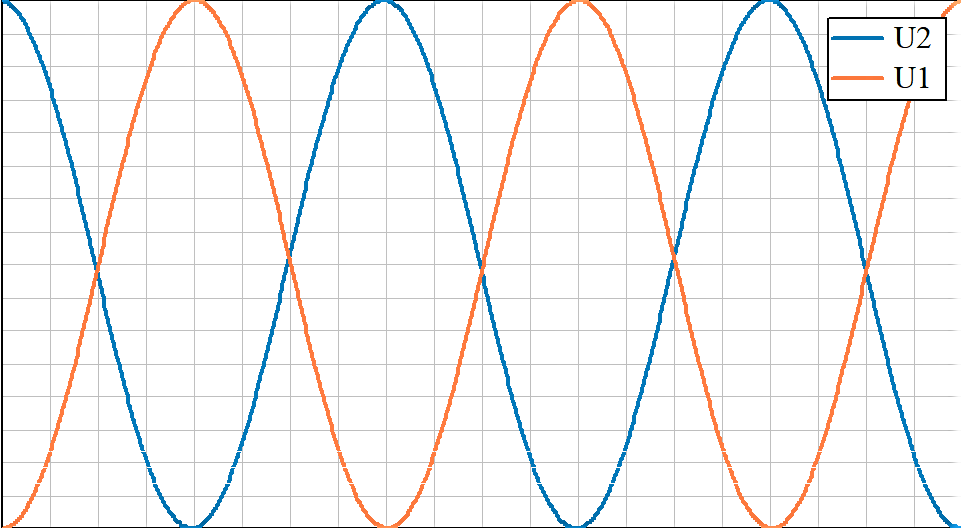
\includegraphics[width=0.4\textwidth]{epur1}}
      \ffigbox[\FBwidth+1cm]{\caption{НМП}}{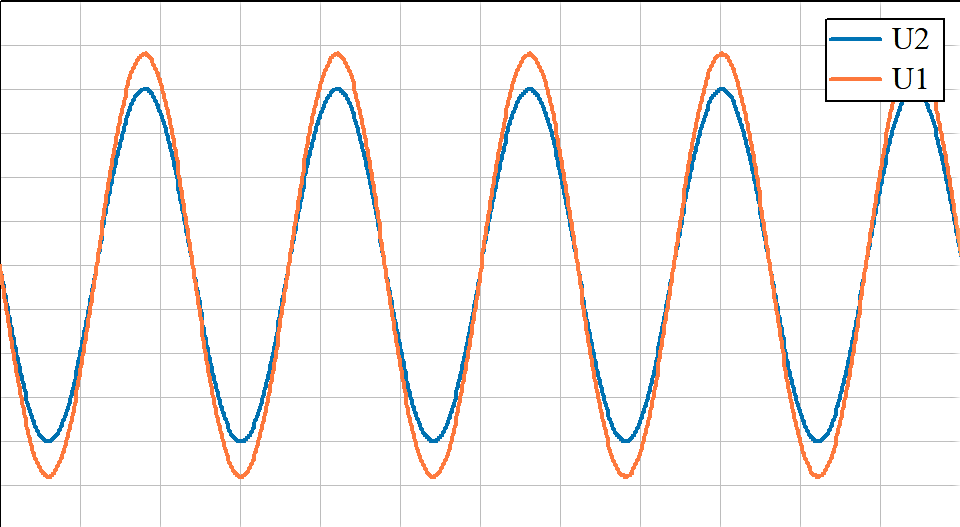
\includegraphics[width=0.4\textwidth]{epur}} 
      
    \end{subfloatrow}
 }
  { % подпись ко всему float 
   \caption{Епюри напруг $U_1$ і $U_2$ підсилювача в схемі}
  }
  \end{figure}


\begin{figure}[h]
\center{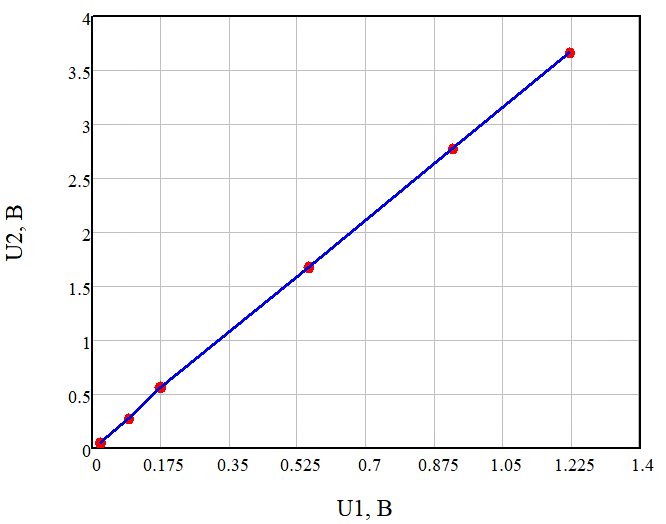
\includegraphics[width=0.6\textwidth]{amp}}
\caption{Амплітудна характеристика НМП}
\end{figure}
\newpage
\begin{figure}[h]
\center{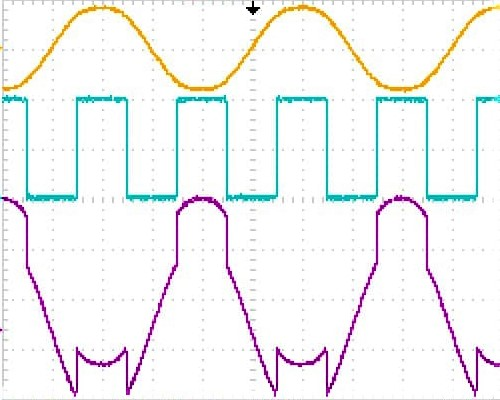
\includegraphics[width=0.3\textwidth]{skotobaza1}}
\caption{Осцилограми $U_{11}(t)$, $U_{12}(t)$, $U_2(t)$ для ДМУ}
\end{figure}

\begin{figure}[h]
\center{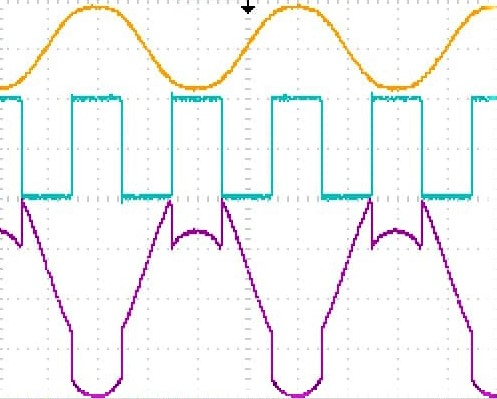
\includegraphics[width=0.3\textwidth]{skotobaza2}}
\caption{Осцилограми $U_{11}(t)$, $U_{12}(t)$, $U_2(t)$ для ИСУ}
\end{figure}


\begin{figure}[h]
\center{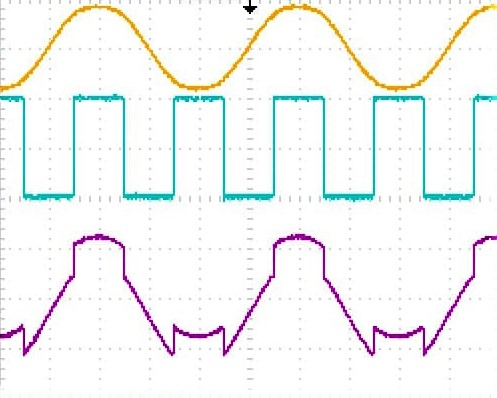
\includegraphics[width=0.3\textwidth]{skotobaza3}}
\caption{Осцилограми $U_{11}(t)$, $U_{12}(t)$, $U_2(t)$ для НСУ}
\end{figure}

\newpage
\begin{center}
{\Large 7.Аналіз результатів та висновки}
\end{center}






%\multirow{объединить Х строк}{ширина}{содержимое}
%\begin{tabular}{|p{6cm}|p{5cm}|p{5cm}|}
%\includegraphics[width=0.5\textwidth]{lablub}
%\medskip\hrule\medskip
%\multicolumn{2}{c|}{Диаметр}

\end{document}